\subsection{用小平板仪测绘平面图}\label{subsec:czjh2-6-12}
\begin{enhancedline}

在兴修水利、规划农田、筑路架桥等基建工程中,常用小平板仪测绘平面图。
下面介绍使用一种比较简单的小平板仪进行测量的原理。

小平板仪是用三脚架支撑的正方形平板,在平板上放图纸用来绘制测出的平面图(图 \ref{fig:czjh2-6-44})。

\begin{figure}[htbp]
    \centering
    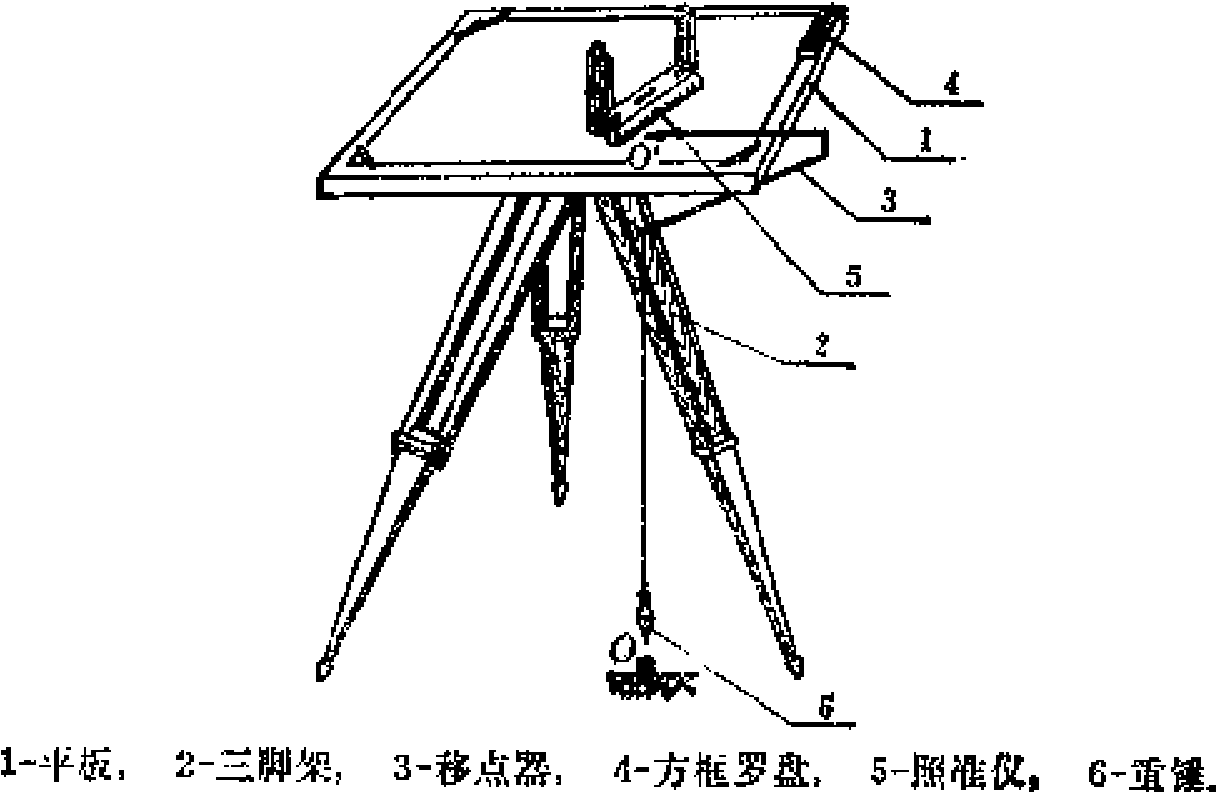
\includegraphics[width=10cm]{../pic/czjh2-ch6-44.png}
    \caption{}\label{fig:czjh2-6-44}
\end{figure}

照准仪是用来观测、绘图的工具(图 \ref{fig:czjh2-6-45})。

\begin{figure}[htbp]
    \centering
    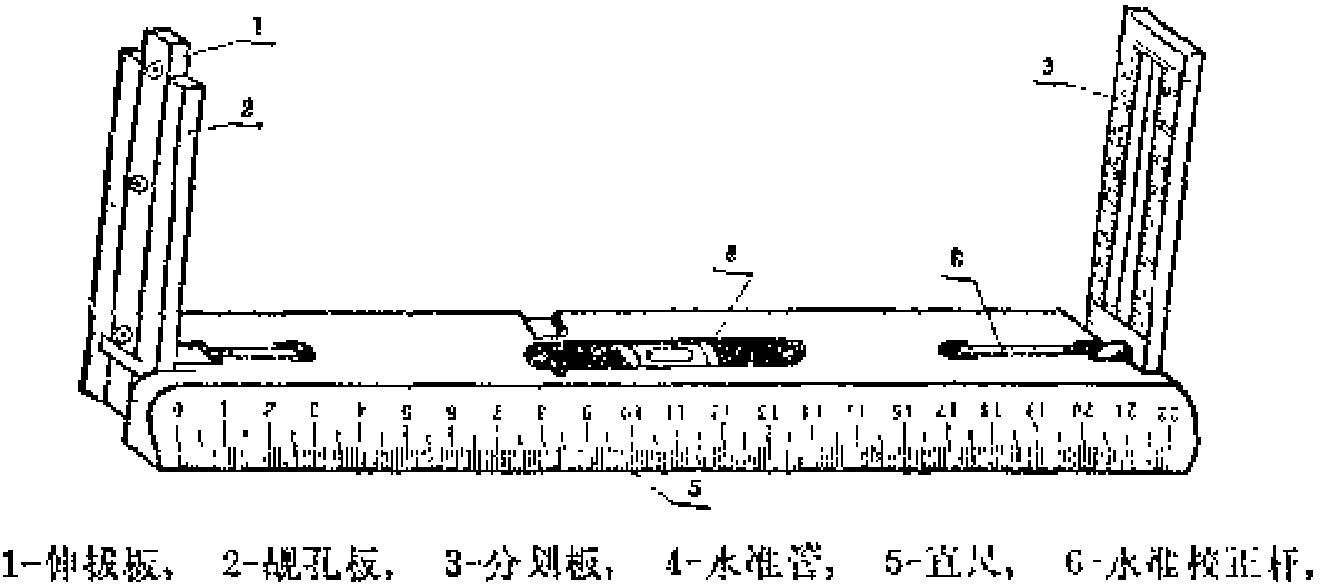
\includegraphics[width=10cm]{../pic/czjh2-ch6-45.png}
    \caption{}\label{fig:czjh2-6-45}
\end{figure}


测绘时还要用到移点器、方框罗盘、标杆、卷尺、测绳等工具。

绘制平面图形,当测绘地区的范围不很大,能够选定测站使它能通视各测点并直接测量出该测站到各测点的距离时,可以使用射线法。

\begin{figure}[htbp]
    \centering
    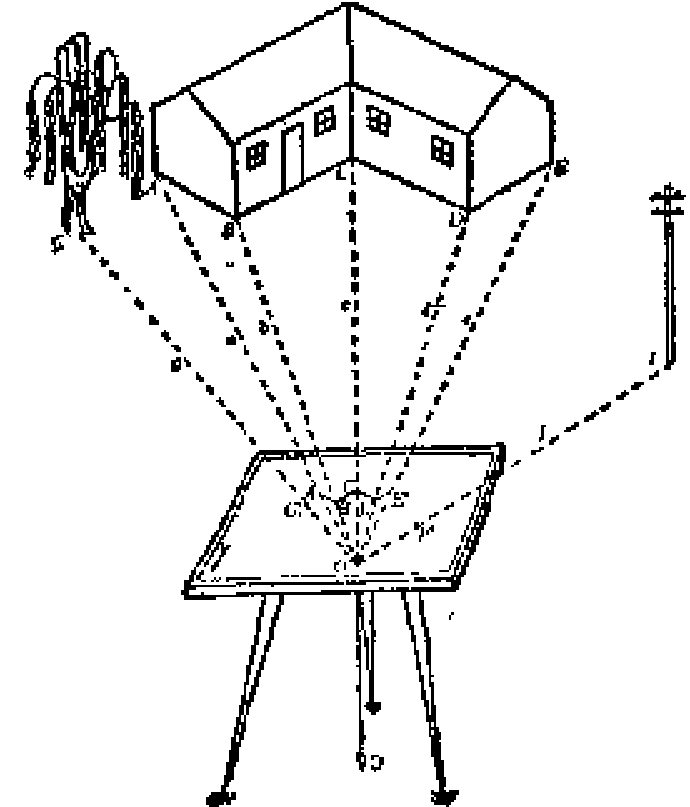
\includegraphics[width=10cm]{../pic/czjh2-ch6-46.png}
    \caption{}\label{fig:czjh2-6-46}
\end{figure}

如图 \ref{fig:czjh2-6-46},在测站 $O$ 安装小平板仪,使平板成水平位置,然后在图纸上标出与点 $O$ 相应的点 $O'$,
测出点 $O$ 与点 $A$ 的距离,再用照准仪在图纸上画出 $OA$ 的方向线 $a$,并按预定的比例尺 $1:k$ 在 $a$ 上画出 $O'A'$。
这样,就在图纸上确定了与测点 $A$ 相对应的点 $A'$。

用同样的方法,可在图纸上测定方向线 $b$,$c$,… 上的与测点 $B$,$C$, … 相对应的点 $B'$,$C'$,…的位置。

所有各测点的位置都在图纸上确定之后,该地区的平面图就可以描绘成了。

如果把上述测绘过程中的图纸上的点 $O'$ 和实际的测站 $O$ 看作为同一个点,那么,
点 $A'$ 和 $A$、$B'$ 和 $B$、 $C'$ 和 $C$、… 的连线都经过同一点,而且
$$ \dfrac{O'A'}{O'A} = \dfrac{O'B'}{O'B} = \dfrac{O'C'}{O'C} = \cdots = \exdfrac{1}{k} \juhao $$
点 $A'$、$B'$、$C'$、… 和点 $A$、$B$、$C$、… 是以点 $O'$ 为位似中心,相似比为 $\exdfrac{1}{k}$ 的外位似对应点。
这样就可以画出比例尺为 $1:k$ 的平面图。

\end{enhancedline}

